\begin{pastexam}[label={px:gw3-112-ds-01}]{關務三等資訊處理 112 年 第一題}
（申論；25 分）

將中序運算式轉換成後序運算式演算法常使用堆疊資料結構，如相同問題，改成使用二元樹資料結構來儲存一中序運算式，以
中序運算式 A/B$-$C+D$*$E$-$A$*$C 為例，畫出表示此中序運算式的二元樹，並依前序（Preorder）與後序（Postorder）列出
拜訪（Visit）此二元樹的順序。（25 分）
\end{pastexam}

\begin{pastsoln}
答案：根是最後一個 $-$；前序 $-$ + $-$ / A B C * D E * A C；後序 A B / C $-$ D E * + A C * $-$。

\textbf{加括號。} $*$、$/$ 優先於 $+$、$-$，同級由左而右結合（資結書第~6.3~節）：
\[
\Bigl(\bigl((A / B) - C\bigr) + (D * E)\Bigr) - (A * C) .
\]
最後才做的運算是最右邊那個 $-$，它是根：左子樹是 $((A/B) - C) + (D*E)$，右子樹是 $A * C$。 左子樹的根是 $+$，再往下
拆成 $(A/B) - C$ 和 $D * E$，依此類推。 運算子都是內部節點、運算元都是葉子（資結書第~7.7~節）：
\begin{center}
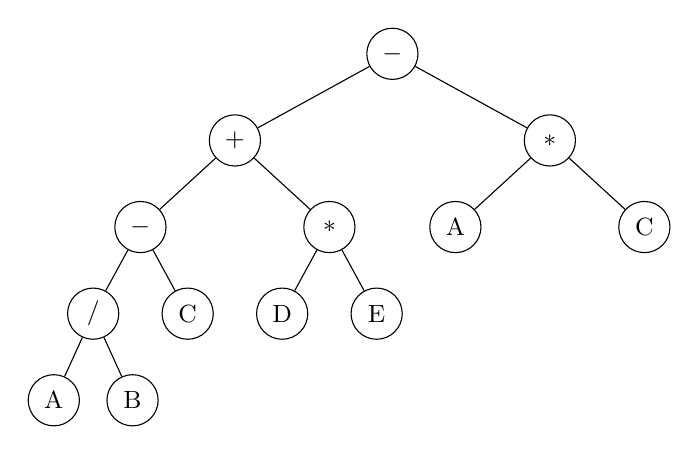
\begin{tikzpicture}[v/.style={circle,draw,minimum size=6.5mm,inner sep=0pt,font=\small},
  level distance=11mm, level 1/.style={sibling distance=40mm}, level 2/.style={sibling distance=24mm},
  level 3/.style={sibling distance=12mm}, level 4/.style={sibling distance=10mm}]
\node[v] {$-$}
  child {node[v] {$+$}
    child {node[v] {$-$}
      child {node[v] {/} child {node[v] {A}} child {node[v] {B}}}
      child {node[v] {C}}}
    child {node[v] {$*$} child {node[v] {D}} child {node[v] {E}}}}
  child {node[v] {$*$} child {node[v] {A}} child {node[v] {C}}};
\end{tikzpicture}
\end{center}
檢查：中序走訪（左、根、右）得 A / B $-$ C + D $*$ E $-$ A $*$ C，和原式相同；每個運算子節點的兩棵子樹就是它的兩個
運算元。

\textbf{走訪}（資結書第~7.3~節）：
\begin{itemize}
\item \textbf{前序}（根、左、右）：先根 $-$，再整棵左子樹（$+$、$-$、/、A、B、C、$*$、D、E），最後右子樹（$*$、A、C）：
\[
-\ +\ -\ /\ A\ B\ C\ *\ D\ E\ *\ A\ C
\]
這就是原式的前序（波蘭）表示法。
\item \textbf{後序}（左、右、根）：
\[
A\ B\ /\ C\ -\ D\ E\ *\ +\ A\ C\ *\ -
\]
這就是原式的後序表示法，和用堆疊做中序轉後序（資結書第~6.3.3~節）得到的結果相同。
\end{itemize}

\textbf{和堆疊轉換的關係。} 題目提到「改成使用二元樹」：建好運算式樹之後，前序、中序、後序走訪分別直接給出前序式、
中序式、後序式，一棵樹可以同時得到三種表示法；後序走訪時遇到運算子就計算它兩個子節點的值，也可以直接求值。 例如
A $= 6$、B $= 2$、C $= 1$、D $= 4$、E $= 5$ 時，值是 $((6/2) - 1) + 20 - 6 = 16$。
\end{pastsoln}
